\chapter{A brief history of molecules}\label{ch:history}

\vspace{-1.5 em}
\minitoc\hrule
\vspace{1.5 em}

What is Coulomb explosion imaging? A technical definition could be given, however, it is simply a decades-old technique in a long line of techniques stretching back centuries, all meant to answer a question posed by the ancient Greeks and Indians---what are the building blocks of the universe, and how do they behave?

It is easy to get stuck in the ivory tower and get lost within the trees of science, losing sight of the big picture of where your research leads.

\section{Atomism: an ancient question}

\section{Seeing molecules: from scientific understanding to saving lives}

\section{Molecular movies}
Molecular movies are of course not only of interest in physics and chemistry as a means of probing fundamental processes, but also in the biological sciences where molecular structure play a crucial role in determining the function of biomolecules such as proteins. However, the molecules of interest there are much too large to be studied by any of the previous techniques. Thus molecular movies in the biological sciences tend to be annotated computer simulations amalgamated from multiple studies. That said, they are very impressive pieces of work.

A particularly impressive movie by \citet{Cheung12} showcases the process of RNA polymerase transcription and goes on for over six minutes.

% FOCUS ON THE HISTORY OF CEI IN DETERMINING GEOMETRIES
\section{Coulomb explosion imaging}
The original CEI experiment is generally traced back to \citet{Vager89} in which the Coulomb explosion is initiated by passing a molecular beam through a thin foil. This is possibly because it was the first work claiming to report a molecular structure, as previous works utilizing CEI do exist, however they mainly report on energy and angle distributions. 

The laser makes its entrance surprisingly early 

There do exist other methods of initiating CEI, for example, single photons from a synchrotron source, x-ray pulses from a free-electron laser, or electron collision.

\subsection{Foil-forged images}
CEI was first performed by \citet{Vager89} whereby the Coulomb explosion was initiated by passing a molecular beam through a thin ($\sim$\SI{30}{\angstrom}) aluminum film at high velocities ($\sim0.02c$). Their work was motivated by the opportunity of imaging non-classical molecular structures that more popular methods were incapble of seeing. They were also the first to suggest that measuring the velocity (or momentum) vectors of each fragment would be provide all the information required to describe the molecule's structure. However, they do not perform any geometry reconstruction and report their fragment ion densities in a coordinate system defined by the asymptotic velocity of each particle, and claim that it is a direct measurement of the square of the multidimensional wave function of a many-body system.

\begin{figure}
  \centering
  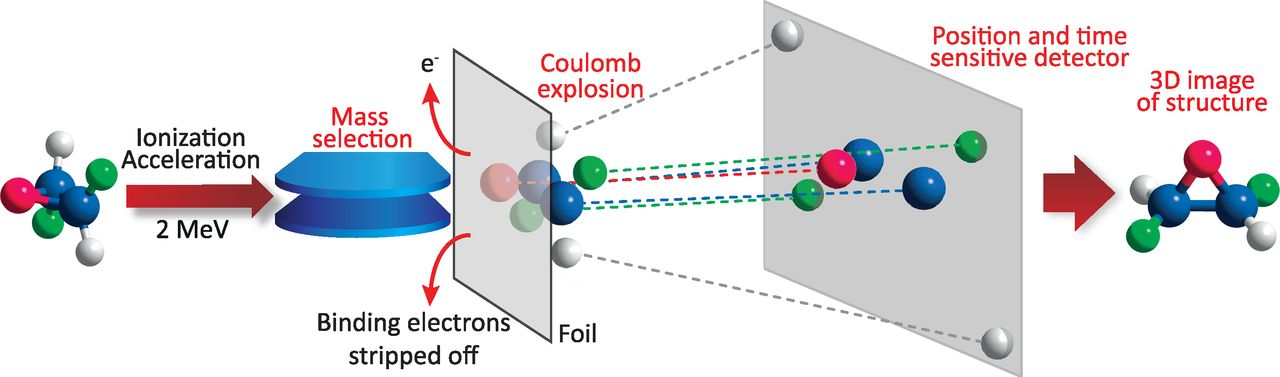
\includegraphics[width=\textwidth]{gfx/FoilExperiment}
  \caption[Schematic of a foil-induced Coulomb explosion imaging experiment.]
  {Schematic of a foil-induced Coulomb explosion imaging experiment. From \citet{Herwig13}. Reprinted with permission from AAAS.}
\end{figure}

One drawback of initiating Coulomb explosions using a thin foil is that a molecular beam must be prepared.

\subsection{CEI by highly charged ion impact}
\subsection{Laser-induced CEI}
\index{Coulomb explosion imaging!History}
\citet{Legare05structure,Legare05dynamics} was the first to use ultrashort laser pulses to induce Coulomb explosion and report on molecular structures and dynamics. To obtain the structures, they assume the explosion proceeds under a purely Coulombic potential and use optimization methods to make guesses at the structure that most accurately reproduces the observed data consistent with minimizing a least-squares objective function. Unfortunately they provide very minimal information regarding their methods and there is a complete lack of discussion acknowledging the shortcomings of this method\footnotemark. Using 8 fs laser pulses they report on the structure of D2O and SO2 \citep{Legare05structure}. They also claim to have imaged vibrating D2+ and dissociating SO22+ and SO23+ however they provide no more than a couple of dissociation frames and infer the transient D2+ bond length from kinetic energy release ratios as a function of pump-probe time delay \citep{Legare05dynamics}.

\footnotetext{The main shortcomings being degenerate solutions and the fact that they employ convex optimization methods to a problem that is not convex. It is not clear if they even knew about these issues.}

\index{Classical imaging formula}
\index{Coulomb explosion imaging!Classical imaging formula}
Surprisingly, an attempt was made to arrive at an analytical solution for calculating geometries from measured momentum data. \citet{Nagaya04} were able to derive a so-called classical imaging formulas giving the position wavefunction squared for the Coulomb explosion of a diatomic molecule and a linear triatomic molecule\footnotemark. They treat the cases of symmetric and asymmetric Coulomb explosion.

\footnotetext{They seem to have worked hard to find an analytical solution but their unsaid conclusion seems to be that it is an intractable problem and their group went silent on this problem.}

\citet{Gagnon08} reported the reconstruction of dichloromethane (CH2Cl2) using a home-made \footnotemark stochastic-based simulated annealing algorithm that globally optimizes the molecular spatial configuration. They discuss uncertainties but are only able to obtain the structure in five cases.

\footnotetext{There is nothing wrong with writing your own code here but nonconvex optimization algorithms are tricky to get right and the reliance should be on professional code.}

\index{Lookup table}
The best effort so far has probably been the one by \citet{Kunitski15} in which they use a lookup table approach to image the elusive Efimov state of the helium trimer.